% Casos de uso esenciales. Fuente: diagramas/tikz/ob2/Ob2_CU_*.tex (bash diagramas/tikz/ob2/build.sh).

\subsubsection{Casos de uso}

Los casos de uso asignan los requerimientos (Tabla~\ref{tab:requerimientos}) a los actores del proceso propuesto. En el sistema de información (Figura~\ref{fig:ob2_cu_sistema}), la secretaria gestiona pacientes, citas y cobros; el odontólogo registra la atención, que incluye el odontograma, los diagnósticos, los tratamientos y la receta; y el director hereda los casos del odontólogo y administra usuarios y catálogos.

\begin{figure}[H]
\centering
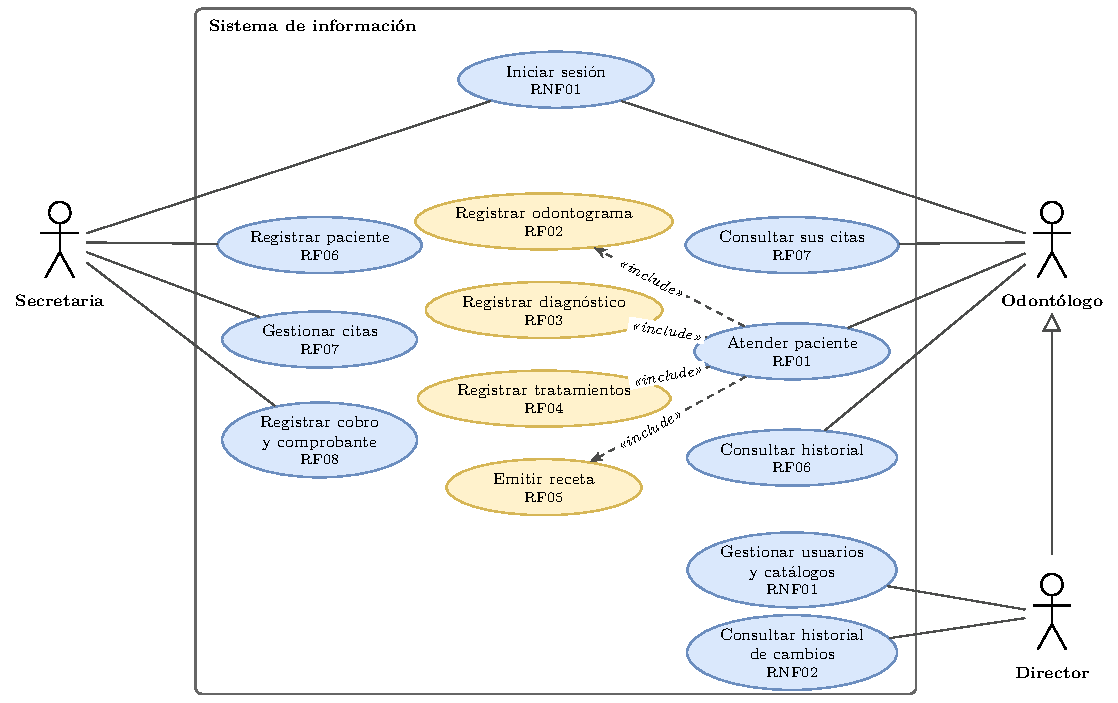
\includegraphics[width=\linewidth]{img/Objetivo2/Ob2_CU_Sistema.pdf}
\caption{Casos de uso del sistema de información}
\label{fig:ob2_cu_sistema}
\end{figure}

En el agente (Figura~\ref{fig:ob2_cu_agente}), el paciente consulta, agenda y responde recordatorios; agendar y reprogramar exigen identificarlo, y lo que el agente no resuelve se deriva a recepción.

\begin{figure}[H]
\centering
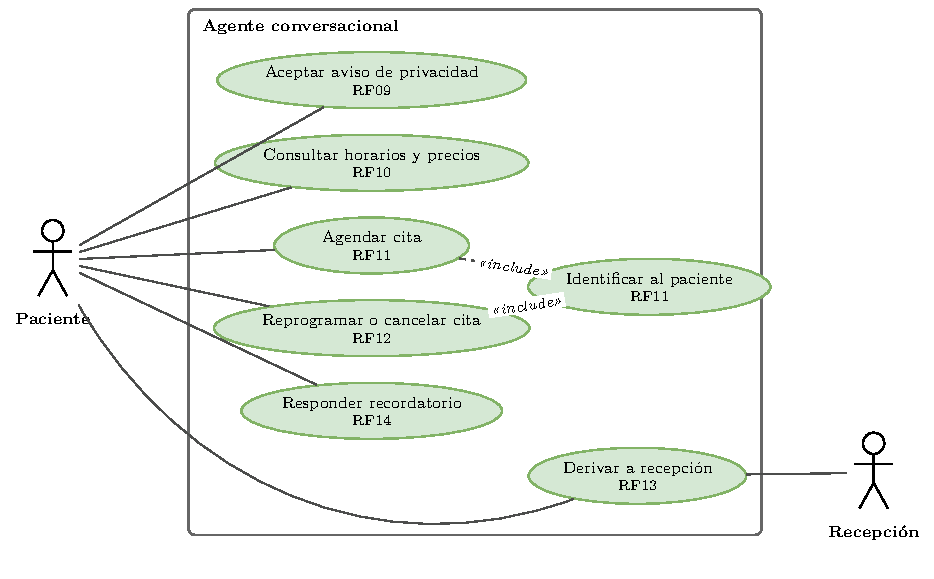
\includegraphics[width=0.9\linewidth]{img/Objetivo2/Ob2_CU_Agente.pdf}
\caption{Casos de uso del agente conversacional}
\label{fig:ob2_cu_agente}
\end{figure}
